\chapter{ArcFace}\label{ch:arcface}
ArcFace~\cite{ArcFace} is a research which became public in 2018 and achieved state-of-the-art results on LFW dataset.

ArcLoss is based on the equation of \textit{softmax loss}~\ref{eq:softmax}.
There are few steps separating the original and the improved version:
\begin{enumerate}
    \item First step is to fix the bias $b_j = 0$.
    \item Then we transform the logit using the dot product definition $W_j^T x_i = \norm{W_j} \norm{x_j} \cos \theta_j$
    $\theta$ is the angle between the weight $W_j$ and the feature $x_i$.
    \item In a third step we fix the individual weights $\norm{W_j} = 1$ by $l_2$ normalization
    \item We do the same for feature $x_i$ and re-scale it to $s$ where coefficient $s$ is predetermined feature scale.
    These normalization steps make the prediction depend only on the angle $\theta$.
    The embeddings are distributed on the hypersphere with a radius $s$.
\end{enumerate}

\begin{figure}[H]
    \centering
    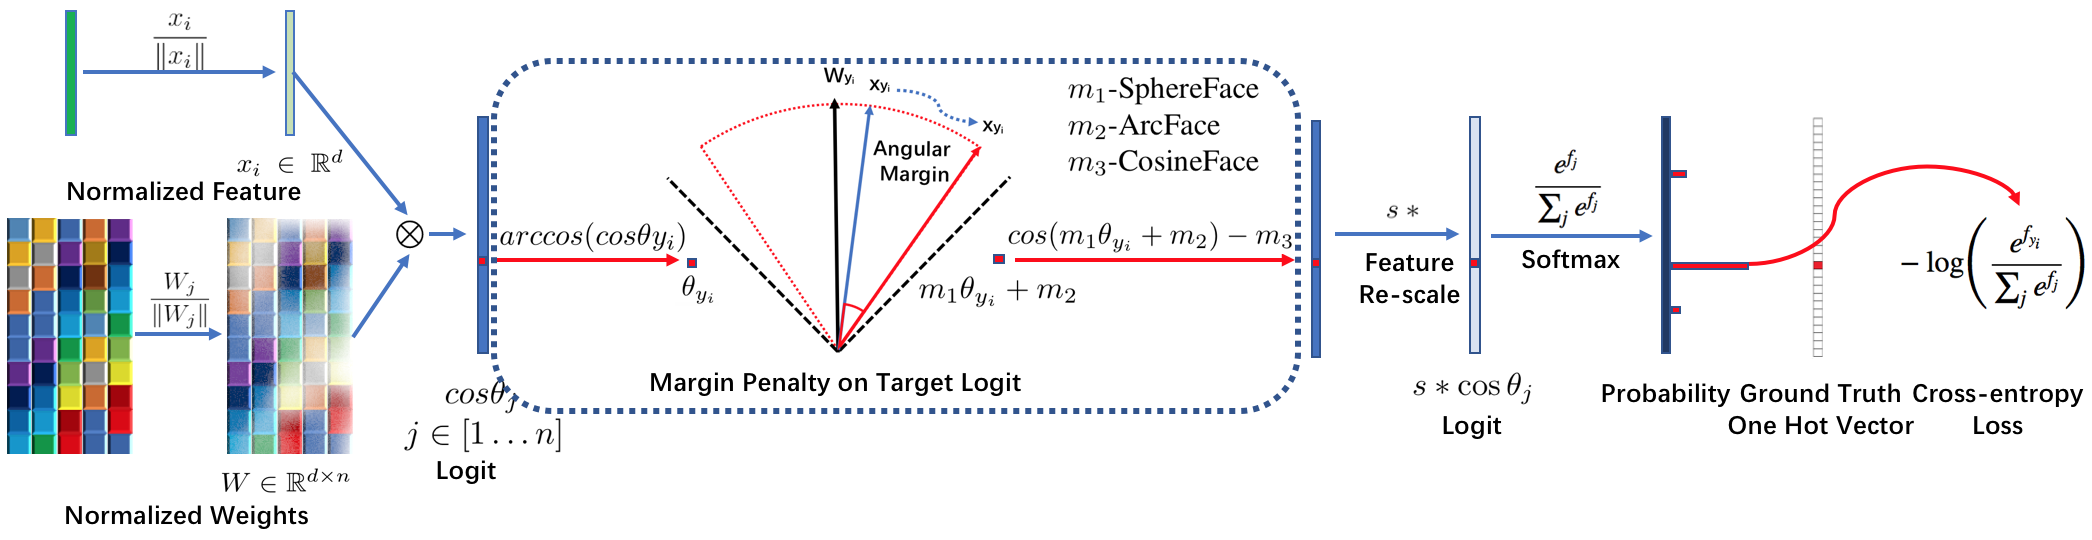
\includegraphics[width=\columnwidth]{images/arcface/arcface.png}
    \caption{Training a CNN for face recognition supervised by the ArcFace loss~\cite{ArcFace}}
    \label{fig:arcface}
\end{figure}

At this point the loss function equation is as follows:
\begin{equation}
    \mathcal{L} = -\frac{1}{N} \sum_{i=1}^{N} \log \frac{e^{s \cos(\theta_{y_i,i})}}
    {e^{s\ \cos(\theta_{y_i,i})} + \sum_{j = 1, j \neq y_i}^n e^{s\ \cos(\theta_{j,i})}}.
\end{equation}

\begin{enumerate}
    \setcounter{enumi}{4}
    \item Now we incorporate the additive margin penalty \textit{m} between $x_i$ and $W_{y_i}$.
    The angluar margin is equal to the geodesic distance\footnote{Distance of a curve representing shortest path
    between two points in a surface.} on the hypersphere which is the reason why the method is called
    \textit{ArcFace}.
\end{enumerate}

Final ArcFace loss function:
\begin{equation}
    \mathcal{L} = -\frac{1}{N} \sum_{i=1}^{N} \log \frac{e^{s \cos(\theta_{y_i,i} + m)}}
    {e^{s\ \cos(\theta_{y_i,i} + m)} + \sum_{j = 1, j \neq y_i}^n e^{s\ \cos(\theta_{j,i})}}.
\end{equation}

\section{Comparison with SphereFace and CosFace}\label{sec:arc-comparison}
By having a look at figure~\ref{fig:arcfacecomp} we can do a comparison of geometric differences of decision margins.
The advantage of \textit{ArcFace} is its constant linear angular margin throughout the whole interval.

\begin{figure}[H]
    \centering
    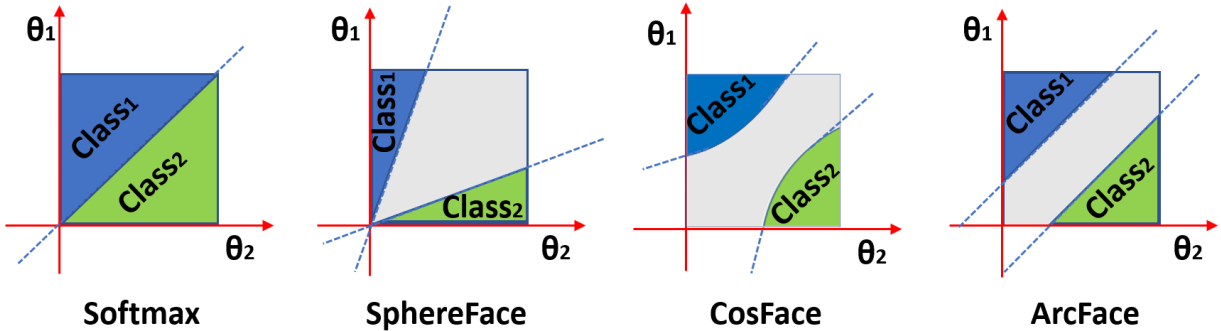
\includegraphics[width=\columnwidth]{images/arcface/arcfacecomparison.png}
    \caption{Decision margins of different loss functions under binary classification case.~\cite{ArcFace}}
    \label{fig:arcfacecomp}
\end{figure}

We can see the concrete results in table~\ref{tbl:arcfacecomp}.
ResNet100 with ArcFace loss trained on MS1MV2~\ref{subsec:ms1m} dataset exceeded the results of methods mentioned in
this thesis.

\begin{table}[H]
    \begin{tabularx}{\textwidth}{l|XXc}
        Method                & \#Image & LFW~\ref{subsec:lfw}            & YTF~\ref{subsec:ytf}            \\ \hline
        FaceNet~\ref{subsubsec:facenet}               & 200M    & 99.63          & 95.10          \\
        Center Loss~\ref{subsubsec:center-loss}           & 0.7M    & 99.28          & 94.90          \\
        SphereFace~\ref{subsubsec:sphereface-loss}            & 0.5M    & 99.42          & 95.00          \\
        CosFace~\ref{subsubsec:cosface}               & 5M      & 99.73          & 97.60          \\
        MS1MV2, R100, ArcFace & 5.8M    & \textbf{99.83} & \textbf{98.02}
    \end{tabularx}
    \caption{Verification performance (\%) of different methods on LFW and YTF datasets.}
    \label{tbl:arcfacecomp}
\end{table}